\chapter{Tools}


\section{Serial Terminal} \hypertarget{def:sterm}{}

To use this tool with PICSimLab you first need to configure a virtual serial port as described in Chapter: \hyperlink{def:seriali}{Serial Communication}.
It is possible to use this tool with a real serial port connected to a real device. 

Open the serial terminal  \href{https://github.com/neundorf/CuteCom}{Cutecom}


\section {Serial Remote Tank} \hypertarget{def:srtank}{}

To use this tool with PICSimLab you first need to configure a virtual serial port as described in Chapter: \hyperlink{def:seriali}{Serial Communication}.
It is possible to use this tool with a real serial port connected to a real device. 

Serial Remote Tank

\begin{figure}[H]
\center
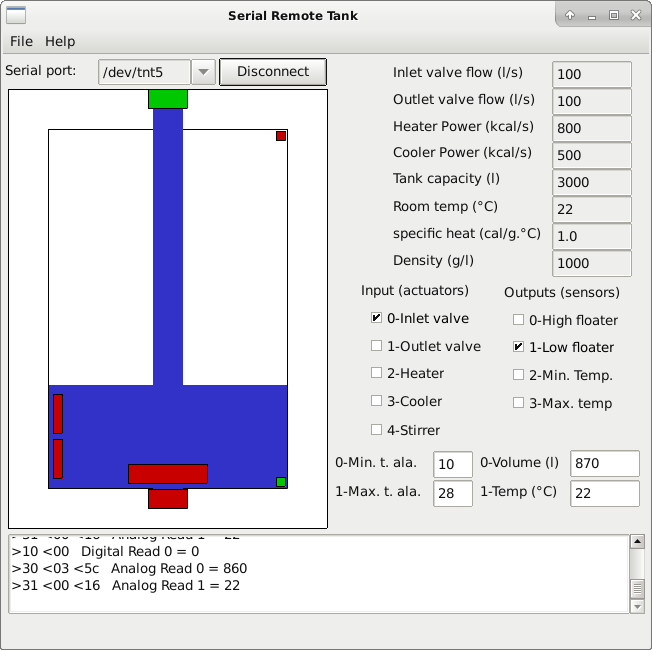
\includegraphics[width=0.8\textwidth]{img/srtank.png} 
\end{figure} 


\subsection{Sensors and Actuators}


\subsubsection{Actuators}

Digital inputs
\begin{enumerate}
\item Inlet valve
\item Outlet valve
\item Heater
\item Cooler
\item Stirrer
\end{enumerate}



Analog inputs
\begin{enumerate}
\item Minimal temperature alarm trigger level
\item Maximal temperature alarm trigger level
\end{enumerate}

\subsubsection{Sensors}

Digital outputs
\begin{enumerate}
\item High floater 
\item Low floater
\item Minimal temperature 
\item Maximal temperature
\end{enumerate}


Analog outputs
\begin{enumerate}
\item Volume
\item Temperature
\end{enumerate}




\subsection{Communication Protocol}


\subsubsection{Writing on Digital Input}
Sent one byte in 0x0N hexadecimal format where N  is the number of input followed by a second byte with value 0x00 for disable or 0x01 for enable.  

Example to turn on the input 2:
\begin{verbatim}
            Serial_write(0x02);
            Serial_write(0x01);
\end{verbatim}


\subsubsection{Reading Digital Output}
Sent one byte in 0x1N hexadecimal format where N  is the number of output and read one byte. The byte readed have value 0x00 for disable or 0x01 for enable. 

Example to read output 3:
\begin{verbatim}
      Serial_write(0x13);
      valor=Serial_read(0);
\end{verbatim}


\subsubsection{Writing on Analog Input} 
Sent one byte in 0x2N hexadecimal format where N  is the number of input followed by two bytes with the 16 bits value.

Example to write the value 230 on analog input 1:
\begin{verbatim}
            Serial_write(0x21);
            valor=230;
            Serial_write((valor&0xFF00)>>8);
            Serial_write(valor&0x00FF);
\end{verbatim}

\subsubsection{Reading Analog Output}
Sent one byte in 0x3N hexadecimal format where N  is the number of output and read two bytes to form the 16 bits value.

Example to read analog output 2:
\begin{verbatim}
      Serial_write(0x32);
      valorh=Serial_read(0);
      valorl=Serial_read(0);
      valor=(valorh<<8)|valorl;
\end{verbatim}



\section{Esp8266 Modem Simulator} \hypertarget{def:espmsim}{}

To use this tool with PICSimLab you first need to configure a virtual serial port as described in Chapter: \hyperlink{def:seriali}{Serial Communication}.
It is possible to use this tool with a real serial port connected to a real device. 

ESP8266 Modem Simulator

\begin{figure}[H]
\center
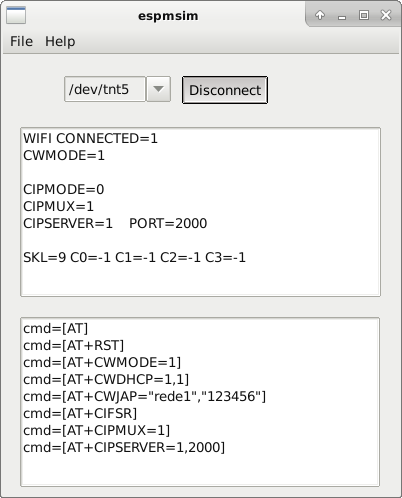
\includegraphics[width=0.7\textwidth]{img/espmsim.png} 
\end{figure} 

\subsection{Supported Commands}

\begin{itemize}
\item AT
\item AT+RST
\item AT+GMR
\item AT+CWMODE=1
\item AT+CWDHCP=1,1
\item AT+CWLAP
\item AT+CWJAP="rede1","123456"
\item AT+CIFSR
\item AT+CIPMUX=1
\item AT+CIPSERVER=1,2000
\item AT+CIPSEND=0,10
\item AT+CIPCLOSE=0
\end{itemize}


\section{Arduino Bootloader}\hypertarget{def:aboot}{}

To use this tool with PICSimLab you first need to configure a virtual serial port as described in Chapter: \hyperlink{def:seriali}{Serial Communication}.

Load microcontroller with Arduino serial bootloader 


\section{MPLABX Debugger Plugin} \hypertarget{def:mpdebug}{}

Open the web page to download the plugin 


\section{Pin Viewer} \hypertarget{def:pinv}{}

 Open the Pin status viewer program. 

 PinViewer connects to PICSimLab through the \hyperlink{def:rcontrol}{rcontrol interface} and allows viewing the status
 and direction of all microcontroller pins. It is also possible to change the state of the digital pins and adjust the
 voltage value on the analog pins configured as input. Pins configured as outputs also show the average value, useful 
 for evaluating the functioning of PWM outputs. 
 
\begin{figure}[H]
\center
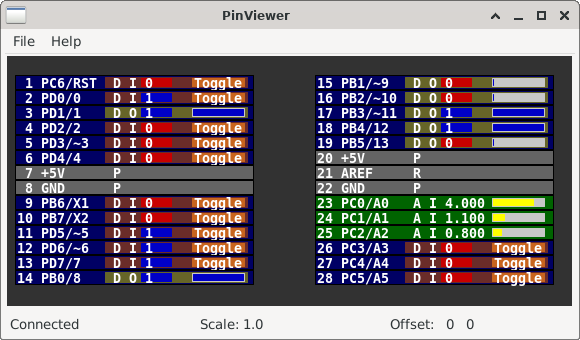
\includegraphics[width=0.7\textwidth]{img/pinviewer.png} 
\end{figure} 
